\documentclass[a4paper,10pt]{article}

\usepackage{fullpage}
\usepackage[spanish]{babel}
\usepackage{cite}
\usepackage[utf8]{inputenc}
\usepackage{a4wide}
\usepackage{url}
\usepackage{graphicx}
\usepackage{caption}
\usepackage{float} % para que los gr\'aficos se queden en su lugar con [H]
\usepackage{subcaption}
\usepackage{wrapfig}
\usepackage{color}
\usepackage{amsmath} %para escribir funci\'on partida , matrices
\usepackage{amsthm} %para numerar definciones y teoremas
\usepackage{hyperref} % para inlcuir links dentro del texto
\usepackage{tabu} 
\usepackage{comment}
\usepackage{amsfonts} % mathbb{N} -> conjunto de los n\'umeros naturales  
\usepackage{enumerate}
\usepackage{listings}
\usepackage{todonotes} % Para poner notas en el medio del texto!! No olvidar hacer. 
\usepackage{framed} % Para encuadrar texto. \begin{framed}
\usepackage{csquotes} % Para citar texto \begin{displayquote}
\usepackage{epigraph} % Epigrafe  \epigraph{texto}{\textit{autor}}

\usepackage{titlesec}


\newtheorem{midef}{Definition}
\newtheorem{miteo}{Theorem}

\definecolor{dkgreen}{rgb}{0,0.6,0}
\definecolor{gray}{rgb}{0.5,0.5,0.5}
\definecolor{mauve}{rgb}{0.58,0,0.82}

\lstset{frame=tb,
  language=Sql,
  aboveskip=3mm,
  belowskip=3mm,
  showstringspaces=false,
  columns=flexible,
  basicstyle={\small\ttfamily},
  numbers=none,
  numberstyle=\tiny\color{gray},
  keywordstyle=\color{blue},
  commentstyle=\color{dkgreen},
  stringstyle=\color{mauve},
  breaklines=true,
  breakatwhitespace=true,
  tabsize=2
}

\title{Aprendizaje autom\'atico}
\author{Grupo Sociof\'isica \\
Sebasti\'an Pinto, Guillermo Pasqualetti, Gustavo Landfried}

\begin{document}

\maketitle

\section{Introducci\'on}

Usamos el lenguaje de progrmaci\'on python. 

Usamos conceptos del libro ``An Introduction to Statistical Learning''~\cite{james_hastie_tibshirani}.

\section{Extracci\'on de atributos}

\begin{comment}
  \begin{figure}[H]
    \centering
    \begin{subfigure}[b]{0.4\textwidth}
      \includegraphics[width=\textwidth]{../Imagenes/artificial_sigmoid_fit}
      \caption{}
    \end{subfigure}
  \end{figure}
\end{comment}

\section{Modelos}

\subsection{SVM}


\subsection{DTC}

\par Con la finalidad de escoger el mejor árbol de desición exploramos 
el desempeño sobre los datos de entrenamiento en una grilla de híper-parámetros.
De entre el total de híper-parametros del modelo decidimos profundizar sobre 
tres que nos parecieron especialmente relevantes:
\begin{itemize}
 \item Profundidad máxima [Valor entero]: Máxima profundidad del árbol de desición. 
 \item Criterio Gini Impurity  Information Gain: función que mide la cualidad 
del ``split''. 
  \item Splitter Best  Random: estrategia usada para elegir el mejor 
``split'' en cada nodo.
\end{itemize}

Los híper-parametros ``Criterio'' y ``Splitter'' no tuvieron un impacto 
significativo en la performance; para ellos escogimos los valores Gini Impurity 
y Best, respectivamente.
El híper parametro ``Profundidad máxima'' tuvo, en cambio, un impacto 
importante sobre el desempeño. La figura siguiente muestra 
la relación funcional entre ambos.

  \begin{figure}[H]
    \centering
    \begin{subfigure}[b]{0.4\textwidth}
      \includegraphics[width=\textwidth]{../imagenes/desempeño-profundiad_arboles}
      \caption{}
    \end{subfigure}
    \label{fig:autovalores}
  \end{figure}


Vemos que el desempeño presenta una fuerte mejora con la profundidad máxima 
permitida al árbol hasta profundidades de 15 a 20 niveles. Luego el desempeño 
prácticamente no crece. Para evitarnos posibles problemas de 'overfitting', 
decidimos limitar en 15 la profundidad de los árboles usados con un desempeño 
correspondiente de 0.982.

\subsection{DTC}


\subsection{NB}

El metodo Naive Bayes no resulto adecuado para este set de datos. El desempeño 
sobre los datos de entrenamiento fue de tan solo 0.524.

\subsection{NB}


\par Decidimos realizar el estudio en un principio para SVM con un subconjunto del dataset original. Del tutorial de \emph{scikit-learn} (CITAR!!!) vimos que el tiempo de ejecución es cuadrático con el número de muestras originales, por lo cual vuelve a este método muy lento de entrenar y validar respecto de los observados anteriormente. De un dataset acotado a 10000 mails (50\% ham - 50\% spam) obtuvimos las eficacias de la figura \ref{fig:svm} para distintos kernels y valores del parámetro C.

\begin{figure}[H]
  \centering
  \begin{subfigure}[b]{0.4\textwidth}
    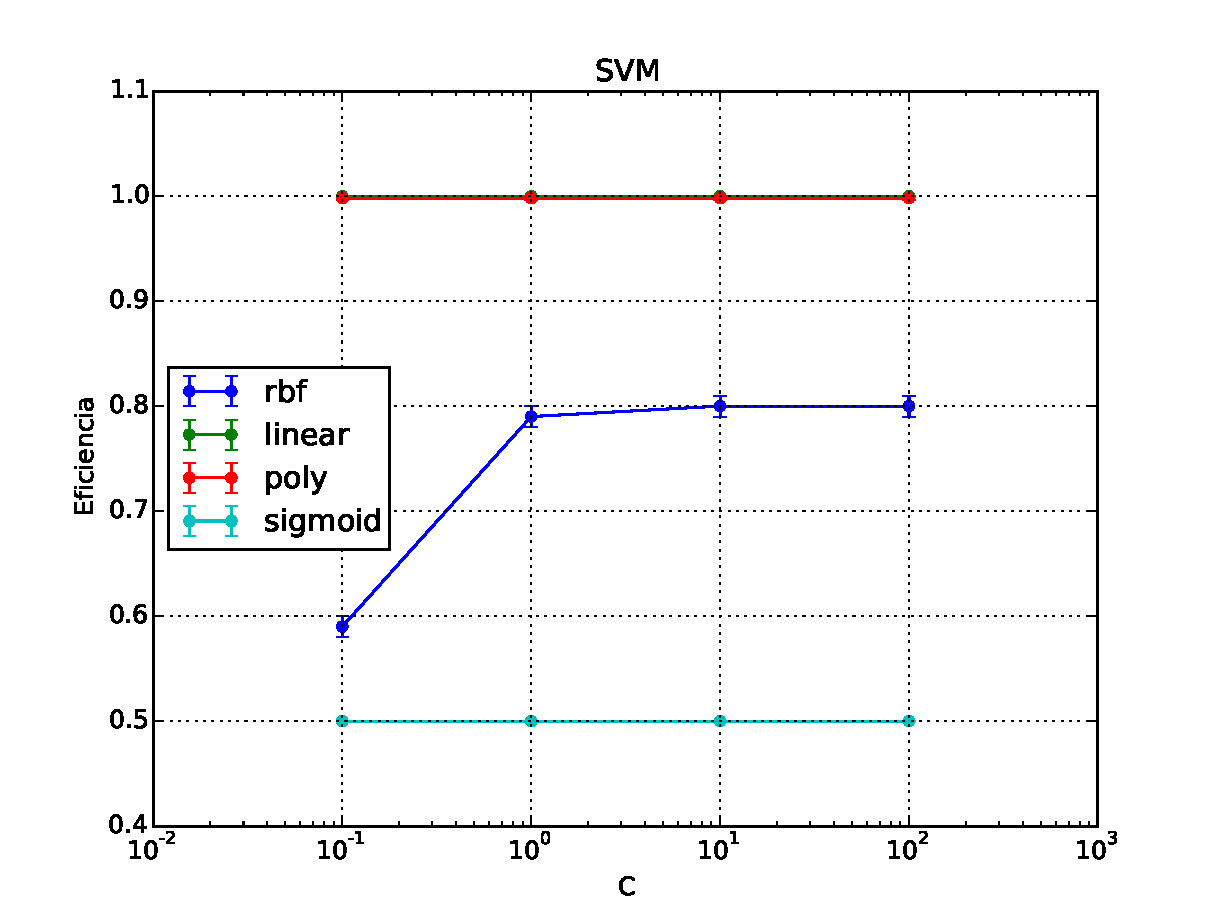
\includegraphics[width=\textwidth]{../imagenes/SVM}
     \caption{}
  \end{subfigure}
  \label{fig:svm}
\end{figure}

(SI TERMINA;, VOY A PONER SVM CON C=1 Y KERNEL = POLY CON TODA LA DATA)

\section{Reducci\'on de dimensionalidad}

\subsection{PCA}

\par De los atributos seleccionados, realizamos un reducción de la dimensionalidad
mediante la técnica de PCA. Dada la matriz de \emph{mails} x \emph{atributos},
calculamos la matriz de covarianza de los atributos, y realizamos una descomposición en valores singulares (SVD). La matriz de covarianza es una matriz simétrica, por lo tanto sus valores singulares coinciden con sus autovalores, que además son reales y no negativos. En la figura \ref{fig:autovalores}, observamos el valor de los mismos, ordenados de mayor a menor. 
  \begin{figure}[H]
    \centering
    \begin{subfigure}[b]{0.4\textwidth}
      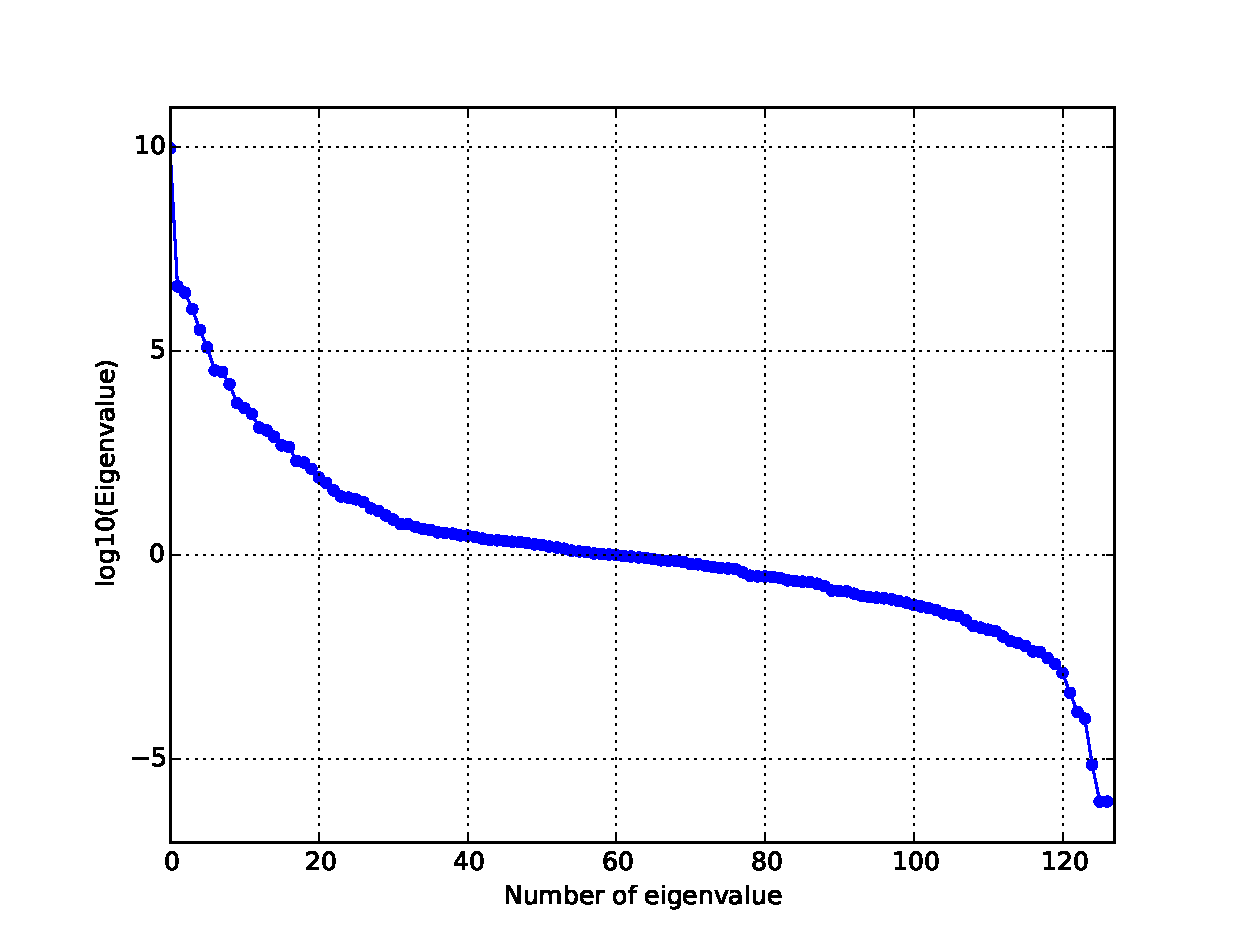
\includegraphics[width=\textwidth]{../imagenes/Autovalores}
      \caption{}
    \end{subfigure}
    \label{fig:autovalores}
  \end{figure}

\par Los autovectores obtenidos de la factorización son una combinación lineal de los atributos elegidos originalmente. Dichos autovectores pueden ser tomados como nuevos atributos, los cuales, a partir de sus autovalores asociados, sabemos en cuáles hay una mayor variabilidad de los datos. Para dar una interpretación a los nuevos atributos, observamos la representación de los autovectores en el espacio de atributos originales. Como criterio, estudiamos qué componentes tienen un valor absoluto mayor a $0.1$ en el espacio de atributos originales. En la tabla \ref{table:autovectores} mostramos el resultado para las 5 direcciones principales. De la tabla vemos que los dos principales atributos coindicen con dos aitrutos originales, mientras los otros tres tienen un grupo de términos, de los cuales el 4 y 5 autovector muestran una correlación más visible entre los miembros del grupo.
\begin{table}
\centering
\caption{}
\label{table:autovectores}
\begin{tabular}{ll}
Autovector & Componentes principales \\
1 & Largo del documento. \\
2 & Cantidad de espacios en blanco. \\
3 & Términos: germ, hi, how, think, valuable, enron, republic, content-class, thread-index. \\
4 & Términos: x-origin, x-filename, x-cc, binary \\
5 & Términos: receive, email, upgrade, fast, spam \\
\end{tabular}
\end{table}


\section{Resultados}

\section{Discusi\'on}


\scriptsize
\bibliographystyle{splncs03}
\bibliography{aa}



\end{document}

